%!TEX root = ../main.tex
\chapter{Compton imaging for a group of UAVs\label{chap:methods_estimation}}
The \ac{MLEM} algorithm for Compton imaging described in the previous chapter has been chosen as a suitable method for data fusion of Compton measurements acquired by a group of \ac{UAV}s.
The motivation for the use of \ac{MLEM} method is described in section \autoref{sec:prelim}.
Section \autoref{sec:setup} presents the adaptation of \ac{MLEM} to the task of online estimation performed by a group of \ac{UAV}s.
The definition of sensitivity and system matrix is described in sections \autoref{sec: sensitivity} and \autoref{sec:system}.

\section{The algorithm of choice}
\label{sec:prelim}
The algorithms for Compton imaging in nuclear medicine (described in the previous chapter) served as inspiration for the imaging method proposed in this thesis.
The algorithm of choice is \acf{MLEM} (more precisely, its list-mode variant for Compton imaging) for the following reasons.

Firstly, the maximum likelihood approach allows us to deal with factors influencing the measurements (such as air attenuation, the distance between the source and the sensor of ionizing radiation,  properties of the sensor and random processes leading to the detection)
as well as cope with the stochastic nature of radioactive emission and model both in a probabilistic way.
It is also a relatively easy-to-apply and time-proven method in the field of nuclear medicine, which has been applied in the robotic sensing of ionizing radiation.

Secondly, the \ac{MLEM} can take into account not only ``positive'' measurements (the Compton events recorded by the sensor) but also ``negative'' measurements (meaning what was NOT measured by the sensor at the given position in space).
Although the radioactive emission, as well as Compton event detection, are stochastic processes, the fact that an \ac{UAV} flew over some position multiple times and did not measure any Compton event is valuable information that might help improve the estimate.
The sensitivity of detection (that is computed during the steps of \ac{MLEM} algorithm) might serve as a map of coverage of the monitored area.
In other words, the sensitivity of detection provides information about how well was which part of the area explored by the drones equipped with the Compton cameras.

Lastly, the algorithm can be easily applied in a scenario with multiple \ac{UAV}s equipped with Compton cameras.
The \ac{MLEM} method is also computationally tractable under some assumptions 
(such as a relatively low number of detected events (which holds for the given scenario and type of sensor) or restriction on the set of possible sources locations)
and can be evaluated online.
The almost real-time estimation is important for active search strategy, where the \ac{UAV}s may adapt their future actions to the current situation.

\section{Online MLEM Compton imaging for group of \ac{UAV}s}
\label{sec:setup}
\subsection{Discretization and hidden parameters}
As described in the chapter \autoref{chap:mlem_theory}, the \ac{MLEM} algorithm belongs to the class of iterative algorithms that work with discretized space of possible source locations.
We assume that the source of ionizing radiation is static and located somewhere on the ground.
We further assume that the \ac{UAV}s are exploring a flat outdoor area without obstacles. Therefore all the potential sources of ionizing radiation are located somewhere on the flat 2D ground plane.

The area of interest (where possible sources of ionizing radiation might be located) is divided into $J$ discrete bins with resolution $r$, each of them is approximated by its centre position and indexed with $j$, $j \in \{1, \dots , J\}$.
The set of all collected measurements (the Compton cones) is denoted $\mathbf{I}$.
The Compton cones are indexed with $i$, $i \in \{1, \dots, I\}$, where $I$ is the total number of cones recorded.
The vector of hidden parameters $\bm{\lambda}\in \mathbb{R}^{J}$ is defined analogously as in the previous chapter, where each element $\lambda_{j}$ represents the expected value of the Poisson distribution, specifying the expected emission rate at position $j$.
The discretization process is illustrated in  \autoref{fig:discretization}.

%multi discretization%%{
\begin{figure}[!h]
  \centering

  \subfloat[area of interest] {
    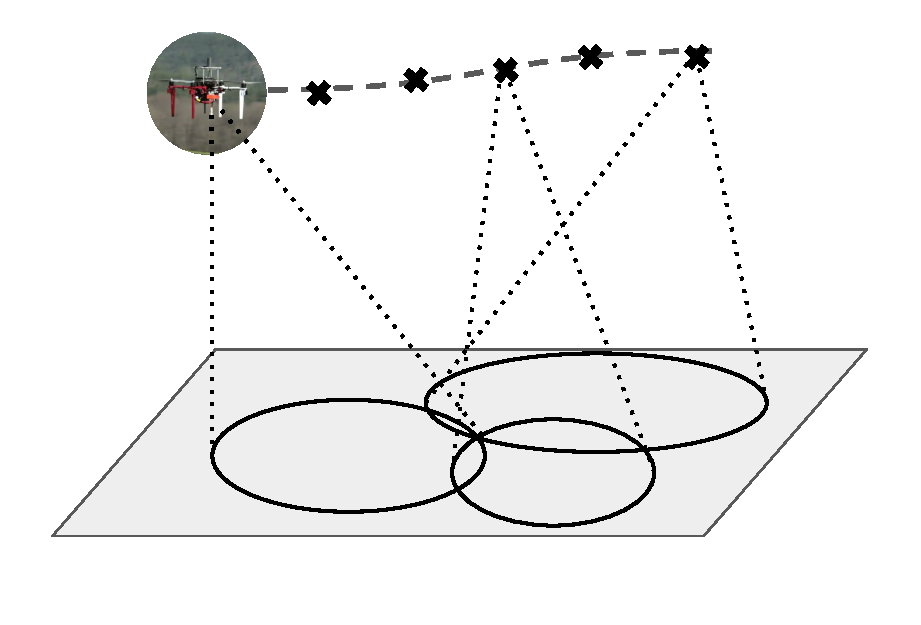
\includegraphics[width=0.32\textwidth]{./fig/photos/dis1.eps}
    \label{fig:dis1}
  }
  \subfloat[area discretized with resolution $r$] {
    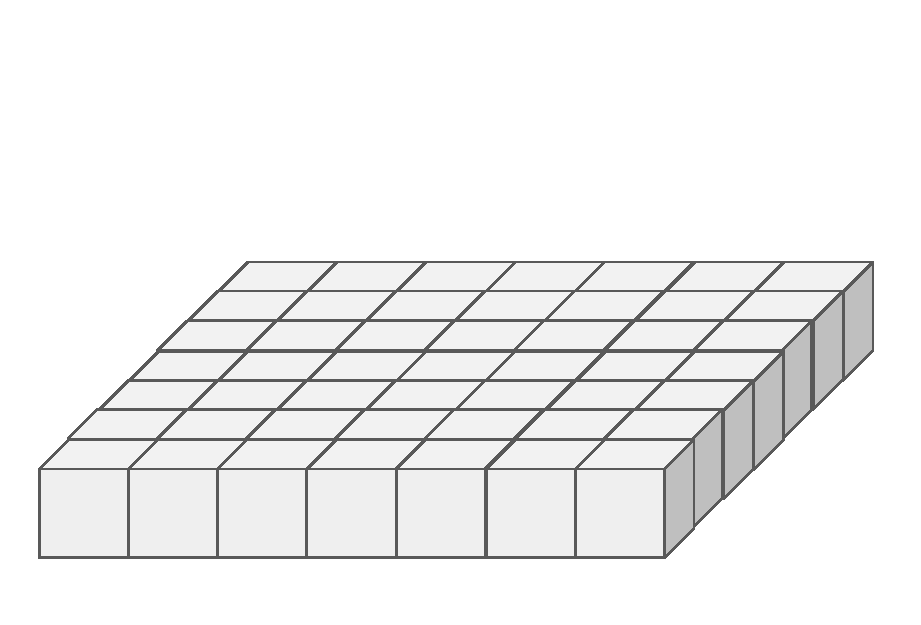
\includegraphics[width=0.32\textwidth]{./fig/photos/dis2.eps}
    \label{fig:dis2}
  }
  \subfloat[hidden parameters $\bm{\lambda}$] {
    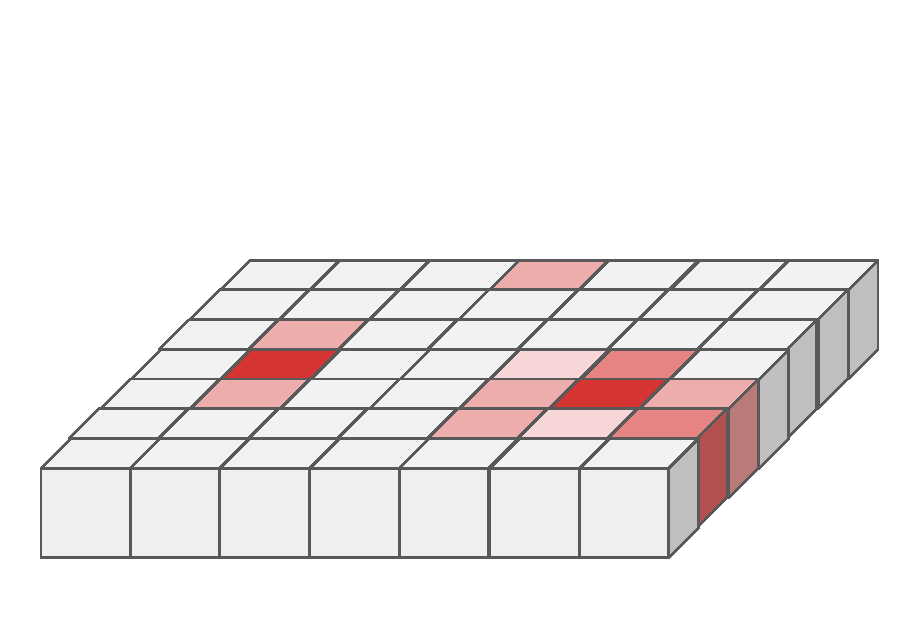
\includegraphics[width=0.32\textwidth]{./fig/photos/dis3.eps}
    \label{fig:dis3}
  }
  \caption{Illustration of the discretization of the space of possible source positions. The open area without obstacles \protect\subref{fig:dis1} is discretized into $J$ discrete bins \protect\subref{fig:dis2}, each represented by its centre position and associated with hidden parameter $\lambda_{j}$ \protect\subref{fig:dis3}.}
  \label{fig:discretization}
\end{figure}% %%}

\subsection{Online maximum likelihood estimation}% %%{
The estimation process proceeds iteratively using the list-mode \ac{MLEM} algorithm:
\begin{equation}
  \lambda_{j}^{[l]} = \frac{\lambda_{j}^{[l-1]}}{s_{j}} \sum_{i \in I} \frac{t_{ij}}{\sum_{k} t_{ik} \lambda_{k}^{[l-1]}},
  \label{eq:MLEM}
\end{equation}
where $l$ is the current iteration of the algorithm, $\lambda_{j}$ is the hidden parameter for each position $j$ we would like to estimate, $t_{ij}$ is the element of system matrix $\mathbf{T}\in \mathbb{R}^{I \times J}$ and $s_{j}$ is the sensitivity of detection for the map position $j$.


As stated before, the \ac{MLEM} algorithm is typically used as an offline method that proceeds all the measurements at once after the end of the experiment.
Medical applications with highly sensitive detectors, together with the short distance between the source and the detector, produce a large number of measurements (tens of thousands and more), and the algorithm typically reconstructs the 3D space with high resolution.
The high number of Compton events results in the fact that the $\mathbf{T}\in \mathbb{R}^{I \times J}$ cannot be stored in the memory during the run of the algorithm and its individual elements $t_{ij}$ are recomputed in every step of the algorithm, which significantly prolongs the computing time.
If the instance of the problem (size of the sampled space $J$ and the number of measurements $I$) is reasonably small, the system matrix $\mathbf{T}$ can be computed only once for each measurement and stored in the memory for future computations, which speeds up the future runs of the \ac{MLEM} algorithm.
Furthermore, the iterations of the \ac{MLEM} algorithm are formulated as matrix multiplication, which allows parallelization using \ac{GPU}.

 \autoref{fig:online_mlem} depicts the workflow of \ac{MLEM} estimation during the experiment.
As the drones fly through the environment, each of the \ac{UAV}s sample its current position at $\SI{5}{\hertz}$.
The sensitivity of detection vector $\mathbf{s}\in \mathbb{R}^{J}$ is updated online based on the newly sampled positions.
Once the new measurement (Compton cone) $i$ is detected, the vector $\mathbf{t}_{i} = [t_{i0}, \dots,t_{ij}, \dots, t_{iJ}]$ is appended to the system matrix.
The iterative \ac{MLEM} algorithm (\autoref{eq:MLEM}) is then repeatedly computed (at $\SI{0.5}{\hertz}$) using currently available sensitivity vector $\mathbf{s}$,  system matrix $\mathbf{T}$ and initialized vector of hidden parameters $\bm{\lambda}$.
The estimate of the distribution of radioactive sources $\bm{\lambda}$ is therefore updated every $2$ seconds, which is technically speaking not in real-time, but the update frequency is sufficient for planning the next actions of the \ac{UAV}s based on the measured data.
%The vector $\bm{\lambda}^{[l=0]}$ is initialized with uniform distribution
%Experiments showed that the proposed approach is computationally tractable for scenarios with an area of size $300 \times 300\ \si{\meter}$ and number 
\mycomment{% %%{
Experiments in simulation and also in real-world showed that the assumption of reasonably small instances holds in practice for the proposed application.
The proposed method is 


The sensitivity vector $\mathbf{s}$ can be iteratively updated during the experiment and with constant memory requirements since the individual elements $s_{j}$ can be updated in place.

The sensitivity vector $S$ is iteratively updated using recorded drone positions that are sampled from drone trajectories (with frequency $\SI{5}\hertz$).
The details of sensitivity computation is provided in section \autoref{sec: sensitivity}.
The system matrix $\mathbf{T}$ is updated (a new row is added) every time a new Compton cone is detected.
The estimation of system matrix $\mathbf{T}$ is described in section \autoref{sec:system}.

The iterative \ac{LM-MLEM} algorithm described in equation \autoref{eq:MLEM} is processed regularly.
The vector of hidden parameters $\mathbf{\Lambda}$ is initialized with cones back-projection.
The \ac{LM-MLEM} estimate is recomputed every $2$ seconds.
}% %%}
% %%}
% melm online%%{
\begin{figure}[htb]
  \centering
    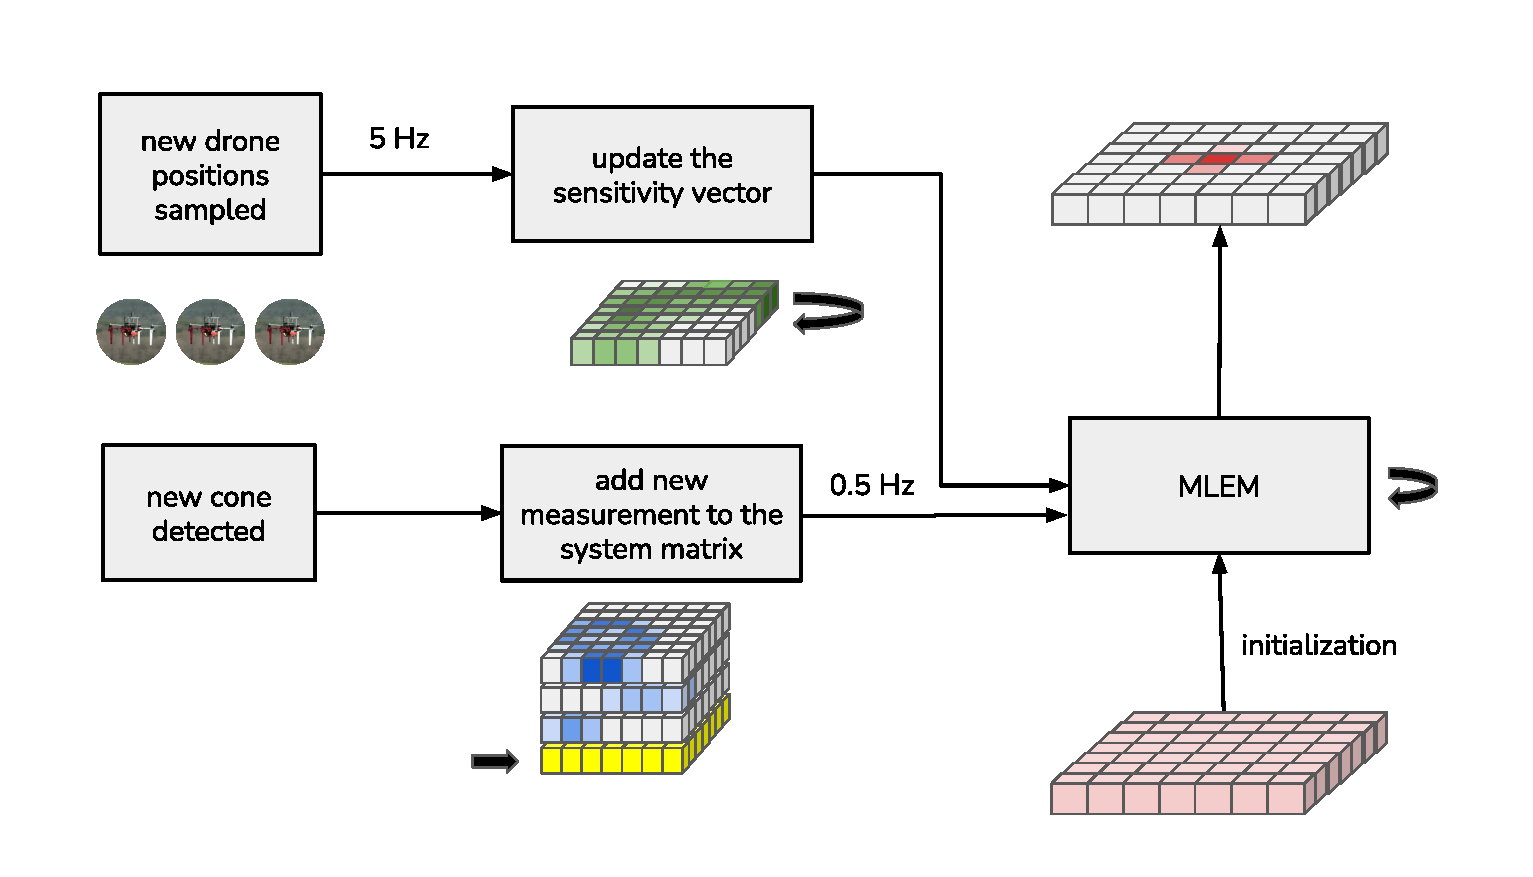
\includegraphics[width=0.99\textwidth]{./fig/photos/workflow.eps}
  \caption{Workflow of the (almost) real-time \ac{MLEM} estimation. The positions of \ac{UAV}s are sampled at $\SI{5}{\hertz}$ and the sensitivity vector $\mathbf{s}\in\mathbb{R}^{J}$ (green) is updated online based on newly sampled positions.
  Once the new Compton cone $i$ is detected by the \ac{pix} Compton camera, 
  the matrix $\mathbf{T}\in\mathbb{R}^{I\times J}$ (blue) is extended by the new vector $\mathbf{t}_{i} = [t_{i0}, \dots,t_{ij}, \dots, t_{iJ}]$ (yellow).
  The iterative \ac{MLEM} algorithm then computes the current estimate of emission intensity $\bm{\lambda}$ (red) every $2$ seconds.
  }
    \label{fig:online_mlem}
\end{figure}% %%}

%Experiments showed that the proposed approach is computationally tractable for real-world scenarios 
%(e.g. autonomous search for multiple compact sources of ionizing radiation of activity $\approx \SI{10}{\giga\becquerel}$ located somewhere in area of size $300 \times 300 \si{\meter}$ discretized with resolution $r = \SI{1}{\meter}$).
%However, there might be scenarios 
%The computational complexity of the \ac{MLEM} algorithm is $\mathcal{O}(I \ J)$, where $I$ is the number of measurements and $J$ is the number of map positions.
%The memory requirements are $\mathcal{O}(I \times J)$
%The scalability of the proposed solution depends on the number of measured Compton cones ($I$) and the size of the area of interest ($J$).
%The number of 
%Experiments showed that the proposed approach is computationally tractable for real-world scenarios 
%(e.g. autonomous search for multiple compact sources of ionizing radiation of activity $\approx \SI{10}{\giga\becquerel}$ located somewhere in area of size $300 \times 300 \si{\meter}$ with sampled with resolution $r = \SI{1}{\meter}$  
%
%The computational feasibility has been tested in simulations and in real-world experiments.

%The sensitivity of detection as well as the system matrix is defined in the following sections.
%The assumption of a reasonably small scenario holds for the proposed application, 
%where the number of recorded Compton cones $I$ is of the order of $10^{3}$ 
%(given low sensitivity and small size of the \ac{pix} sensor) 
%and size of the discretized mapped area $J$ of the order of $10^{5}$  (e.g. area of $300 \times 300 \si{\meter}$ with resolution $r = \SI{1}{\meter}$).

\section{Sensitivity of detection}% %%{
\label{sec:sensitivity}
The probability of a photon emitted from a given position $j$ to be detected by the Compton camera is called the sensitivity of detection.
In the proposed scenario, the sensitivity of the detection can be seen not only as the property of a single Compton camera, but as a sensitivity of the whole multi-robot system, where multiple Compton cameras (mounted on the \ac{UAV}s) are moving through the environment.
The sensitivity can be expressed using conditional probability as 
\begin{equation}
  s_{j} =  P(\textrm{detected by the sensor}\ | \textrm{emitted from } j).
\end{equation}
A series of random occurrences should happen for a photon to be detected by the Compton camera.
First of all, the photon must be emitted from position $j$ towards the sensor surface (emitted under the solid angle subtended by the visible camera surface at the position of the source), not being absorbed by the air along the way.
Then the photon should interact with the matter of the sensor in form of Compton scattering.
%The angle under which it scatters can be described by the Klein-Nishina \cite{Klein-Nishina cross-section.
The scattered photon then must be absorbed by the camera in the form of a photoelectric effect.
This model is simplified because other random occurrences might happen --- for example, the photon might undergo Compton scattering twice in a row, the incident photon might be immediately absorbed, etc.
However, we will stick to the proposed simplified model with particles undergoing Compton scattering and then photoelectric absorption consecutively.

The position of the Compton camera sensor is not static in this case. 
The \ac{UAV}s carrying the Compton camera are dynamically moving through the environment, with varying speed, position and orientation.
Therefore, the positions of the \ac{UAV}s are sampled in time from \ac{UAV}s trajectories and denoted as $v$, where $v \in \{0, \dots , V\}$ and $V$ is the total number of viewpoints generated by all \ac{UAV}s during the experiment.
The sensitivity of detection is evaluated for each $(j,v)$ pair. % %%}

\begin{figure}[!h]
  \centering
    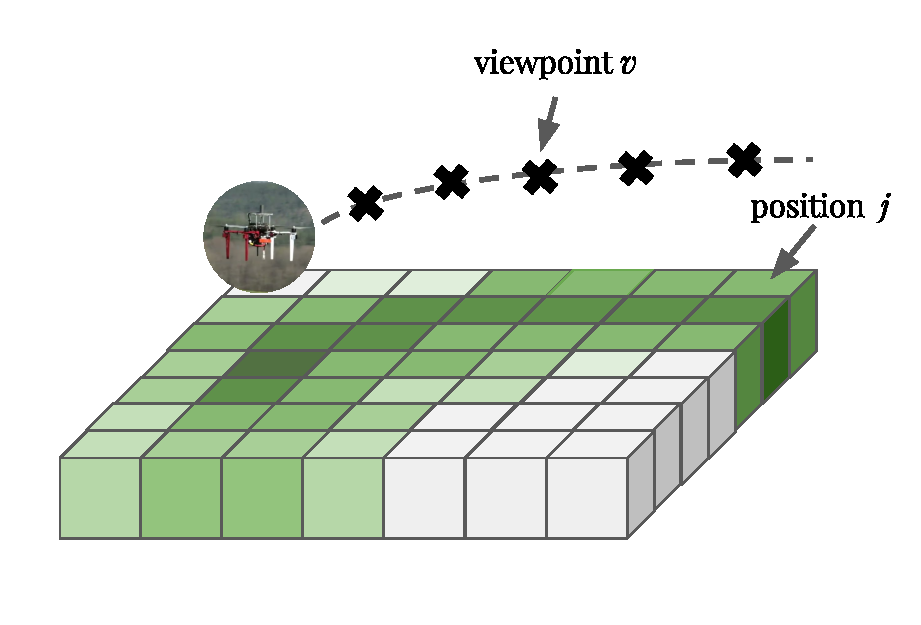
\includegraphics[width=0.6\textwidth]{./fig/photos/sen.eps}
    \label{fig:sen_illustration}
  \caption{An illustration of sensitivity computation. 
  The sensitivity describes the probability that a particle emitted at a given position is measured by the Compton cameras onboard the \ac{UAV}s. 
  In other words, the sensitivity $s_{j}$ describes how well explored has been the map position $j$ during the experiment. 
  The trajectory of the \ac{UAV} is sampled into viewpoints denoted as $v$.
  The sensitivity vector $\mathbf{s}\in\mathbb{R}^{J}$ is illustrated as 2D object just for visualization purposes, although it is a one-dimensional vector.}
\end{figure}% %%}

\subsection{Probabilistic description}% %%{
The series of random occurrences for a photon emitted at position $j$ leading to the detection by the Compton camera at camera position $v$ can be described as follows:
\begin{equation}
  s_{jv} =  (p_{solid\ angle})(1-p_{air})(p_{compton})(p_{absorption}),
  \label{eq:sen_prob}
\end{equation}
where $p_{solid\ angle}$ is the probability that the photon is emitted under the solid angle subtended by the visible camera surface (at position $j$), 
$p_{air}$ is the probability that a photon is absorbed by the air along the way from emission towards the sensor, 
$p_{compton}$ is the probability that Compton scattering occurs, and $p_{absorption}$ denotes that scattered photon is absorbed by the detector and measured.

The literature describes several analytical models for computing the sensitivity of the detection. 
For example, \cite{wilderman2001} proposed a sensitivity model for multi-layer Compton cameras close to the source.
Authors of \cite{maxim2016} proposed a simplified model for Compton cameras with negligible size compared to the distance from the source.
However, these models are not suitable for the problem tackled in this thesis since the multi-layer Compton camera has different properties than the single-layer Compton camera \ac{pix}.
Multi-layer Compton cameras are typically measuring only particles coming from certain directions (from the front side of the camera, perpendicular to its layers).
On the other hand, the \ac{pix} sensor used in this project can potentially measure particles coming from all directions.
The sensitivity of the sensor w.r.t. different directions of the incoming particle is unknown and presents a scientific question that needs to be answered to make the \ac{MLEM} estimate accurate. 

Another option presented in the literature is the evaluation of sensitivity using the Monte Carlo simulation.
This approach has multiple advantages: it is not necessary to describe all random occurrences inside the detector analytically (which might be complicated and take non-negligible computation time when evaluating a large number of map positions during the experiment).
Monte Carlo simulation can be precomputed in advance, and the data can be stored in some data structure that allows fast access to the data, shortening the computation time.
Since it is difficult to describe  equation \autoref{eq:sen_prob} for \ac{pix} Compton camera in analytical form 
(because the probability $p_{compton}$ and $p_{absorption}$ depends on the length of the corresponding intersection of the photon's trajectory with the matter of the detector),
we approximate the terms $(p_{solid\ angle})$, $(p_{compton})$ and $(p_{absorption})$ using the Monte Carlo simulation.% %%}

% sensitivity%%{


\subsection{Monte Carlo simulation}% %%{
The idea of Monte Carlo simulation is simple:
instead of deriving analytical expression,
%which might be complicated given the nature of the \ac{pix} detector (where all interactions are happening in a single block of matter, and probabilities of \ac{CS} or \ac{PE} depend on the length of the ray segment inside the sensor) and time-consuming for online computations during the experiment,
we will approximate the probabilities by simulating sources of ionizing photons at certain positions and compute how many particles emitted there produced Compton cones in the simulated sensor.
The realistic Compton camera simulator described \cite{baca2019timepix} was used as a template and adapted for this particular application.
% \autoref{fig:polar} shows the polar coordinate system, where angles $\theta$ and $\phi$ determine the relative position of the source with respect to the Compton camera.

The position of each simulated source is parametrized by its polar coordinates (angles $\theta$, $\phi$ and distance $d$), as shown in  \autoref{fig:polar}.
Each simulated source emits $N$ particles (in all directions).
Since the \ac{CdTe} semiconductor crystal inside the \ac{pix} sensor is a symmetrical object, only $\frac{1}{8}$ of the elementary sphere around the sensor needs to be simulated.
 \autoref{fig:sources_loc} shows the positions of simulated sources, and  \autoref{fig:sampling} presents their positions in the angle space.
We compute the probability of producing a Compton cone for a particle emitted by a source at the relative position given by polar coordinates ($\theta, \phi, d$) as
\begin{equation}
  p(\mathrm{cone\ detection})_{(\theta, \phi, d)} = \frac{C_{(\theta, \phi, d)}}{N},
\end{equation} 
where $C_{(\theta, \phi, d)}$ is the number of photons that have undergone the Compton scattering and were consecutively absorbed inside the \ac{pix} (the \ac{CdTe} block). 
We also check if the produced interactions passed outlier detection. %and passed the outlier detection (therefore, can be detected).
The outlier detection consists of the minimum pixel distance of the two recorded interactions on the Timepix chip and energy bounds for a recorded electron with energy $E_{1}$ and photon $E_{2}$. 
$N$ is the number of all particles emitted at source position $(\theta, \phi, d)$. 
Number of emitted particles is set to $N = 10^{10}$, the distance $d$ is set to $d = \SI{1}\meter$ for simplicity.
The simulation process is described in algorithm ref{alg:monte}. 
The results of the simulation are stored in a lookup table:
\begin{equation}
  \mathrm{lookup\_table}(\theta_{k}, \phi_{k}) = p(\mathrm{cone\ detection})_{(\theta_{k}, \phi_{k}, d = \SI{1}\meter)}. 
\end{equation}
The lookup table is a data structure that allows a fast readout of the stored data.
For arbitrary query ($\theta, \phi$), the lookup table finds the closest key pair ($\theta_{k}, \phi_{k}$) in the angle space and returns the value associated with the key pair.% %%}

%multi montecarlo
\begin{figure}[!h]% %%{
\centering
  \subfloat[\centering Sampling of the $\frac{1}{8}$ of the unit sphere in the angle space] {
    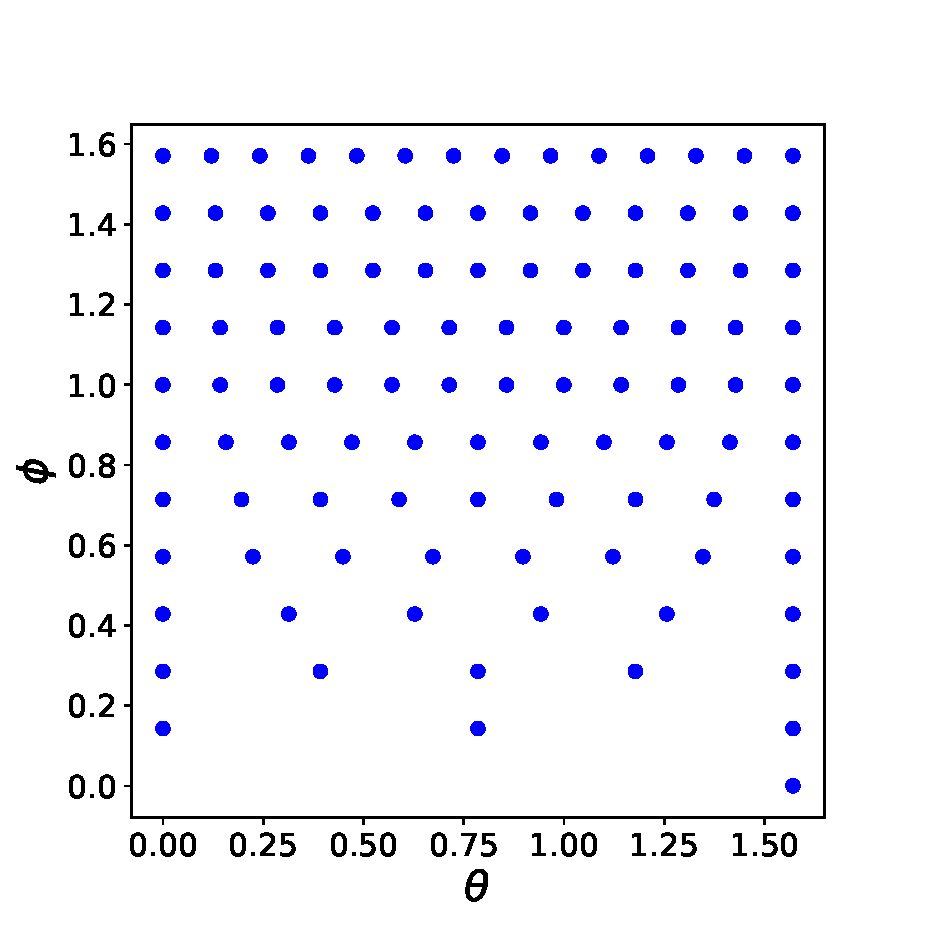
\includegraphics[width=0.3\textwidth,trim={0 0 1cm 1cm}, clip]{./fig/photos/mc_angle_space.eps}
    \label{fig:sampling}
  }
  \subfloat[\centering Locations of the simulated sources] {
    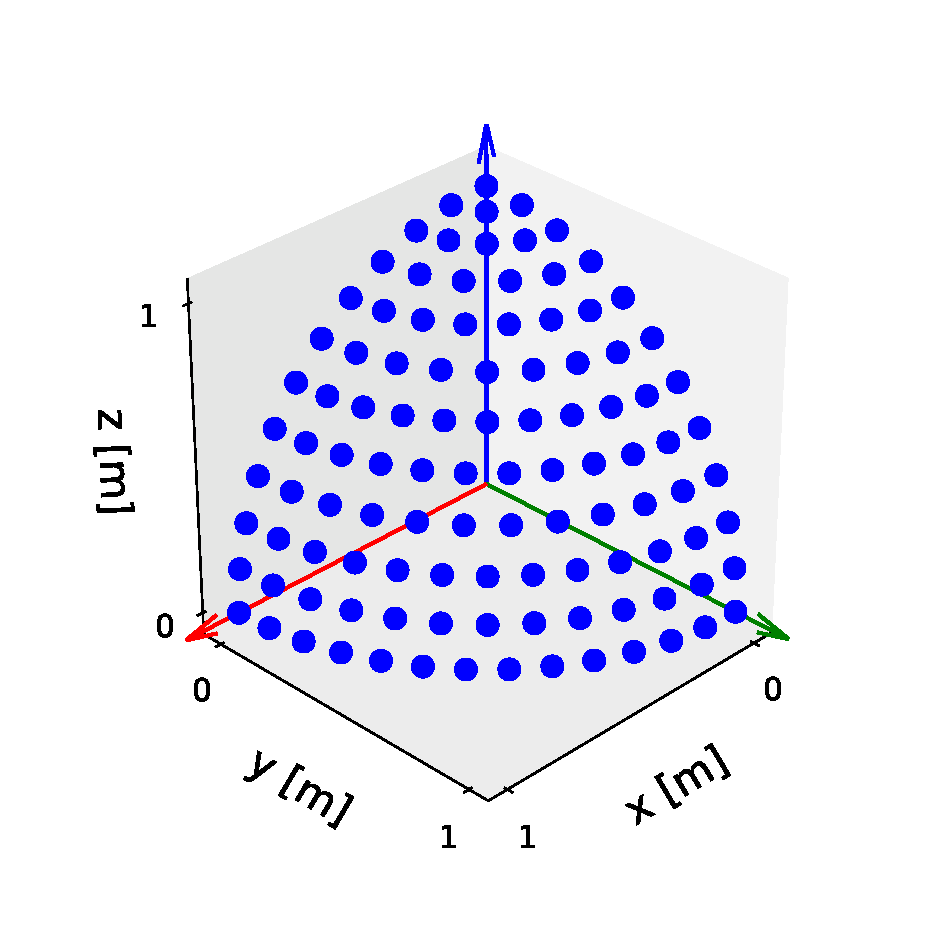
\includegraphics[width=0.3\textwidth, trim={0 0.5cm 2cm 1cm},clip]{./fig/photos/mc_sources.eps}
    \label{fig:sources_loc}
  }
  \newline
  \noindent
  \subfloat[\centering Polar coordinates] {
    \centering
    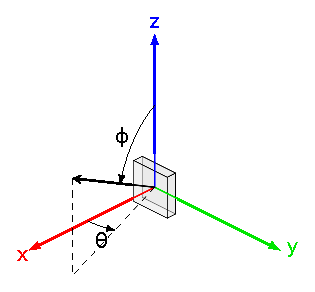
\includegraphics[width=0.25\textwidth]{./fig/photos/axes.eps}
    \label{fig:polar}
  }
  \subfloat[\centering Illustration of the solid angle definition] {
    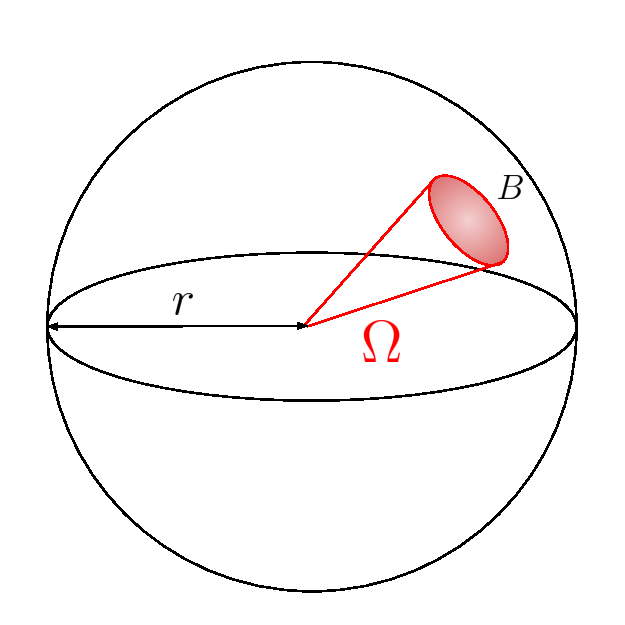
\includegraphics[width=0.25\textwidth]{./fig/photos/solid_angle_2.eps}
    \label{fig:sa}
  }
  \caption{Sampling of $\frac{1}{8}$ of the unit sphere for the Monte Carlo simulation is illustrated in \protect\subref{fig:sampling} (angle space) and \protect\subref{fig:sources_loc} (xyz coordinate system). 
  The polar coordinates determining the direction of incoming particle are presented in \protect\subref{fig:polar}. 
  Finally, the solid angle definition $\Omega = \frac{B}{r^{2}}$, where $r$ is the sphere radius and $B$ is the spherical surface area, is shown in \protect\subref{fig:sa}. }
  \label{fig:mc_multi}
\end{figure}% %%}

%%%%%%%%%%% ALGORITHM %%%%%%%%%%%%%%%%%% %%{
%%%%%%%%%%%%%%%%%%%%%%%%%%%%%%%%%%%%%%%%%%%

%\begin{algorithm}[h!]
%\caption{Monte-carlo simulation}\label{alg:cap}
  \begin{figure}
\begin{algorithmic}
\Function {create\_lookup\_table}{$N$}
  \For {$\theta \in (0, \dots ,\frac{\pi}{2})$}
    \For {$\phi \in (0, \dots , \frac{\pi}{2})$}
      \State $\mathrm{lookup\_table}(\theta, \phi) \gets \Call{compute\_probability}{\theta, \phi, N}$
    \EndFor
  \EndFor
\EndFunction
\Statex
\Function {compute\_probability}{$\theta, \phi, N$}
\State $C \gets 0$
\State $A \gets N\frac{\Omega_{\theta, \phi, d}}{4 \pi}$ \Comment{how many of $N$ particles hits the sensor}
\State $a \gets 0$
\While {$a<A$} 
  \If {\Call{is\_cone\_measured}{$\theta, \phi$}} \Comment{Compton cone measured}
  \State $C \gets C + 1 $ 
  \EndIf
  \State $a \gets a + 1$
\EndWhile
  \State \Return $C/N$ 
  \EndFunction
\Statex
  \Function{is\_cone\_measured}{$\theta,\phi$}
  \State $ray \gets \Call{sample\_sensor\_surface}{\theta,\phi}$ \Comment{ray inside the sensor after hitting its surface}
  \If{\Call{is\_Compton\_scattering}{$ray, E_{0}$}} \Comment{sample if \ac{CS} occured}
  \State $new\_ray, E_{1}, X_{1} \gets \Call{compton\_scattering}{ray, E_{0}}$ %\Comment{Sample }
  \Else{}
    \State \Return False \Comment{No Compton scattering occurred}
  \EndIf
  \If{\Call{is\_photoelectric\_effect}{$new\_ray, E_{1}$}} \Comment{Sample if \ac{PE} occurred} 
    \State $E_{2}, X_{2} \gets $\Call{photoelectric\_effect}{$new\_ray, E_{1}$}
  \Else{}
    \State \Return False
  \EndIf
  \If{\Call{passed\_outlier\_detection}{$E_{1}, E_{2}, X_{1}, X_{2}$}}  \Comment{pixel dist. and energy bounds}
    \State \Return True   
    \Else{}
    \State \Return False
  \EndIf
\EndFunction
\end{algorithmic}
      \caption{The Monte Carlo simulation pseudocode. For each $\theta, \sigma$ pair, the Monte Carlo method first computes the number of particles emitted towards the visible surface of the detector from the current position ($A$) out of all simulated particles ($N$). 
    Then a point for each of $A$ photons is randomly sampled somewhere on the visible sensor's surface, which determines the trajectory of incident photon inside the \ac{CdTe} sensor's block. 
    The Monte Carlo method counts the number of photons ($C$) that fulfilled all the following conditions: a) were emitted under the solid angle of the visible sensor's surface, 
    b) undergone the Compton scattering, 
    c) the scattered photon was absorbed, 
    d) the recorded interactions passed the outlier detection filter.
    The final probability $\frac{C}{N}$ is then stored in the lookup table.}
\label{alg:monte}
\end{figure}
%  \label{alg:monte}
%  \caption{Monte-carlo simulation}
%\end{algorithm}
%%%%%%%%%%%%%%%%%%%%%%%%%%%%%%%%%%%%%%%%%%%% %%}
\newpage
\subsection{Sensitivity computation}% %%{
The sensitivity of detection by the sensor placed at sampled position $v$ for map position $j$ is computed as:
\begin{equation}
  s_{jv} = \underset{(1-p_{air})}{\underbrace{e^{-(\mu d_{jv})} }} \underset{(p_{solid\ angle})\\(p_{compton})\\(p_{absorption})} {\underbrace{\frac{\mathrm{lookup\_table}(\phi_{jv}, \theta_{jv})}{d^{2}_{jv}}}},  
  \label{eq:sjv}
\end{equation}
where $d_{jv}$ is the Euclidean distance between map position $j$ and sensor position $v$, $\mu \approx \SI{0.01}{\meter^{-1}} $ is the linear attenuation coefficient for $\SI{622}{\kilo\electronvolt}$ photons in air, ($\phi_{jv}, \theta_{jv}$) are the polar coordinates determining the relative position of $v$ and the sensor. 
The term $\frac{1}{d^{2}_{jv}}$ in \autoref{eq:sjv} ensures that the $p_{solid\ angle}$ (already contained in the $\mathrm{lookup\_table}$ for $d = \SI{1}\meter$) approximately holds even for distances other than $d = \SI{1}\meter$.

\subsubsection{Iterative formula}
The equation \autoref{eq:sjv} presents the sensitivity computation for one viewpoint $v$. 
However, we would like to compute the sensitivity of detection online during the experiment for all the viewpoints previously recorded. % while keeping the memory requirements constant. 
Therefore the sensitivity vector is iteratively updated with the newly sampled viewpoints (\ac{UAV} positions).
Let denote $\mathbf{s}^{[t]}$ the sensitivity vector at time $t$.
The initial value of $\mathbf{s}^{[0]}$ is initialized with zeros. %$0$ ($s_{j}^{[0]} = 0 ,\forall s_{j}^{[0]} \in \mathbf{s}^{[0]}$).
Let us denote $V^{[t:t+1]}$ the set of viewpoints that were newly sampled between time $t$ and $t+1$ and needs to be processed. 

The sensitivity vector $\mathbf{s}^{[t+1]}$ with elements $s_{j}^{[t+1]}$ is computed as follows:
\begin{equation}
  s_{j}^{[t+1]} = s_{j}^{[t]} + \sum_{v \in V^{[t:t+1]}} s_{jv} \Delta_{v}, 
  \label{eq:sen_iter}
\end{equation}
where the sum $\sum_{v \in V^{[t:t+1]}}$ iterates over all newly processed viewpoints, 
the term $\Delta_{v} = t_{v} - t_{v-1}$ expresses the time difference between current viewpoint $v$ sampled at time $t_{v}$ and its predecessor (previous viewpoint generated from the trajectory of the same \ac{UAV}) sampled at time $t_{v-1}$. 

This formulation of sensitivity has multiple advantages.
Firstly, the memory requirements for storing the vector $\mathbf{S}$ remain the same during the whole experiment. The values $s_{j}$ are updated in place.
Secondly, the sensitivity is updated online as new sampled trajectories of the \ac{UAV} arrive. Therefore the computation time scales well with the increasing duration of the experiment.
Lastly, it takes into account the time difference between sampled viewpoints $\Delta_{v}$.% %%}

%%%%%%%%%%%%%%%%%%%%%%%%%%
%%%%%%%%%%%%%%%%%%%%%%%%%%
%%%%%%%%%%%%%%%%%%%%%%%%%%
\section{System matrix}
\label{sec:system}
The system matrix $\mathbf{T} \in \mathbb{R}^{I \times J}$ is defined as
\begin{equation}
t_{ij} =  P(\textrm{detected in } i | \textrm{emitted from } j).
\end{equation}
In other words, it says how likely the photon causing measurement $i$ came from the map position $j$.
The illustration of the system matrix is depicted in  \autoref{fig:sys_ilustration}, where the blue colour represents $t_{ij}$ values of the individual cells. 
\begin{figure}[!h]
  \centering
    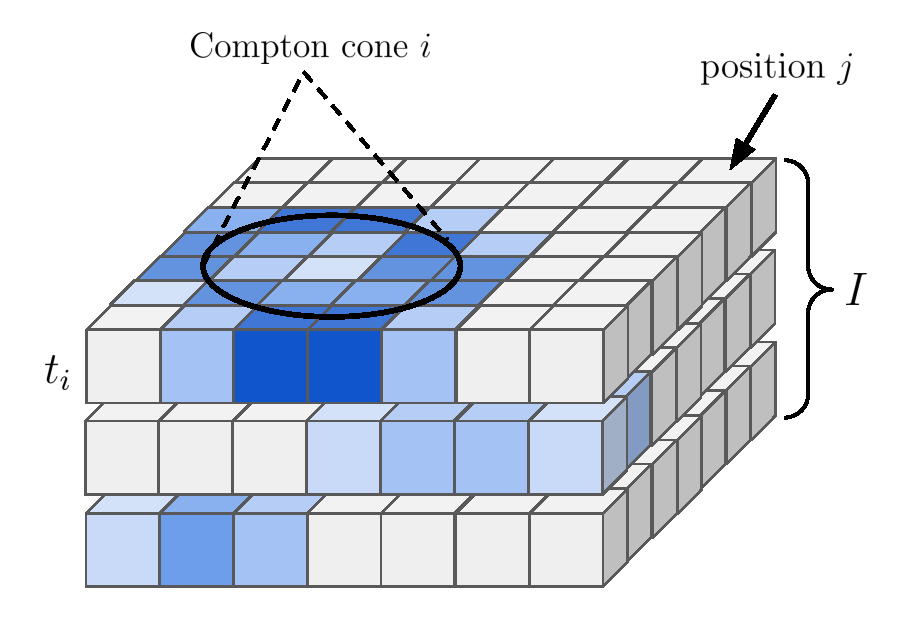
\includegraphics[width=0.48\textwidth]{./fig/photos/systemmmm.eps}
  \caption{System matrix $\mathbf{T}$. The blue colour represents the value of $t_{ij}$ in each cell. The system matrix is visualized as 3D matrix just to highlight the relation with newly measured cone $i$, although it is a two-dimensional matrix of size $I \times J$, where $I$ is the number of recorded Compton cones and $J$ is the size of the map. }
    \label{fig:sys_ilustration}
\end{figure}

%The main question remains the same as for the sensitivity computation: how to evaluate the system matrix for a given scenario and \ac{pix} sensor?

The measurement $i$ is composed of multiple components:
\begin{equation}
  i_{full} = (\beta_{i}, v_{i}, a_{i}, X_{1}, E_{1}, X_{2}, E_{2}),
\end{equation}
where:
\begin{itemize}
  \item $\beta_{i}$ is the reconstructed Compton angle,
  \item $v_{i}$ is the 3D pose (position and orientation) of the sensor in world coordinates at the time when the event was recorded,
  \item $\mathbf{a}_{i}$ is the axis vector of the reconstructed Compton cone,
  \item $X_{1}$ is the position of the first interaction (Compton scattering) inside the detector,
  \item $E_{1}$ is the measured energy of the electron that was created as a side product of the Compton scattering,
  \item $X_{2}$ is the position of the second interaction (absorption) inside the detector,
  \item $E_{2}$ is the measured energy of the absorbed electron.
\end{itemize}
%The first interaction (electron produced as a side product of \ac{CS}) at position ${X_{1}}$ with measured energy $E_{1}$) 
%and the second interaction (absorbed electron at position $X_{2}$ inside the sensor with measured energy $E_{2}$).
%The Compton cone $i$ with scattering angle $\beta_{i}$ is then reconstructed from these measurements using equation \autoref{eq:theta}.
%The position of the sensor at the time when the Compton effect was measured is denoted $v_{i}$ (and is composed of position and orientation in the world coordinates).

\subsection{Probabilistic description}
A series of random occurrences should happen for a photon emitted at position $j$ with initial energy $E_{0}$ to be detected by the Compton camera as measurement $i$.
The term $t_{ij}$ can be described with probabilities as:
\begin{itemize}
  \item $p_{solid\ angle}(j, v_{i}) $: the probability that the photon is emitted at position $j$ under the right solid angle towards the visible surface of the detector at position $v_{i}$,
  \item $(1-p_{air}(d_{jv_{i}}))$: the probability that the photon reaches the detector surface (not being absorbed along the way, where $d_{jv_{i}}$ is the distance from $j$ to detector pose $v_{i}$),
  \item $\bar{p}_{compton}(j, X_{1}, E_{0}, \beta_{i})$: the probability that it interacts with the matter of the detector at position $X_{1}$ and undergo Compton scattering under angle $\beta_{i}$ while losing energy $E_{1}$ to the electron that is immediately measured by the detector,
  \item $\bar{p}_{absorption}(X_{1}, X_{2}, E_{0}, E_{1})$: the probability that the scattered photon interacts with the matter of the detector at position $X_{2}$, is absorbed and energy $E_{2}$ is measured by the detector during the absorption.
\end{itemize}
Same as in the sensitivity section, the presented model is simplified, and several assumptions are made. 
It is assumed that the first interaction is a Compton scattering and the second interaction is the photoelectric effect (absorption) (which might not always be true since other interactions might occur), it is assumed that $E_{0} = E_{1} + E_{2}$, etc.
Unlike in sensitivity computation (where $s_{j}$ describes the probability that a photon emitted from $j$ is detected anywhere by the detectors), the elements of system matrix $t_{ij}$ describe the probability that a photon emitted from $j$ was recorded in measurement $i$, therefore $p_{compton}\neq \bar{p}_{compton}$ and  $p_{absorption}\neq \bar{p}_{absorption}$.

\subsection{Inspiration from literature}
The nuclear medicine literature provides multiple models for the system matrix, such as \cite{wilderman}. 
However, the model is designed for two-layer Compton camera and for scenarios where the detector size is relatively large compared to the distance to the source. Therefore, the geometry of the Compton camera must be considered.
Work presented in \cite{maxim2016} described a simplified model for the Compton camera, which size is negligible compared to the distance to the source of radiation (for two-layer Compton camera).
The energy measurement uncertainties are approximated using Gaussian distribution.
Both of these models do not take into account the effect of environmental attenuation.
Despite all of these differences, it served as an inspiration for the proposed approach.

\subsection{Simplifications of the problem}
Efficient evaluation of $\bar{p}_{compton}$ and $\bar{p}_{absorption}$ is challenging since it depends on the length of the incoming and scattered ray inside the detector.
In the given scenario, the size of the \ac{pix} detector is negligible ($14 \times 14 \times 2 \ \mathrm{mm}$) compared to the distance between the detector mounted on the \ac{UAV} (flying at least $\SI{3}\meter$ above the ground) and source of radiation.
Because of that, modelling $p_{solid\ angle}$ (probability that the particle reaches the detector) and $p_{air}$ (air attenuation) is relatively more important than the accurate modelling of probabilities of events inside the detector.

The following simplification is made:
The measurement $i$ is represented as
\begin{equation}
  i = (\beta_{i}, v_{i}, a_{i})
\end{equation}
and the measured energies and exact positions of interactions inside the detector are ignored,
the Compton camera detector is approximated as a single point with position and orientation $v_{i}$.
However, the probability of detecting the Compton effect produced by particles incoming from some direction is not uniform for all directions (given the non-uniform shape of the sensor).
The lookup table from the previous section (representing the chance that a particle incoming from a specific direction cause any detectable Compton effect, not just the one measured in $i$) is used to approximate the direction sensitivity of the detector.

\subsection{System matrix computation}
The elements $t_{ij}$ of system matrix $\mathbf{T}$ are computed as:
\begin{equation}
  t_{ij} = \underset{(1-p_{air})}{\underbrace{e^{-(\mu d_{jv_{i}})}}}\ 
  \underset{\bar{p}_{compton}} {  \underbrace{K(\beta_{i}, E_{0})\ h(\delta_{ij}|\sigma, \alpha_{ij})}} \
  \underset{(p_{solid\ angle})\\(p_{compton})\\(p_{absorption})} {\underbrace{\frac{\mathrm{lookup\_table}(\phi_{jv}, \theta_{jv})}{d_{jv_{i}}^{2}}}}
  ,%s_{jv} = \underset{(1-p_{air})}{\underbrace{e^{-((\mu/\rho) d_{jv})} }} \underset{(p_{solid\ angle})\\(p_{compton})\\(p_{absorption})} {\underbrace{\frac{\mathrm{lookup\_table}(\phi_{jv}, \theta_{jv})}{d^{2}_{jv}}}},  
  \label{eq:system_matrix_full}
\end{equation}
where:
\begin{itemize}
 \item $d_{jv_{i}}$ is the Euclidean distance between the map position $j$ and sensor position $v_{i}$, 
\item $\mu \approx \SI{0.01}{\meter^{-1}} $ is the linear attenuation coefficient for $\SI{622}{\kilo\electronvolt}$ photons in air\item $K(\beta_{i}, E_{0})$ is the Klein-Nishina formula representing the probability of Compton scattering under estimated angle $\beta_{i}$ for an incoming particle with energy $E_{0}$,
\item $h(\delta_{ij}|\sigma_{j})$ is a Gaussian kernel (the ``blurring factor'') representing the uncertainty in angle measurement,
\item $\delta_{ij}$ is angle difference $|\beta_{i}-\beta_{j}|$, where $\beta_{j}$ is the angle between cone axis vector $a_{i}$ and vector $|j-v_{i}|$, 
\item $\sigma$ is standard deviation and $\alpha$ is the minimal angle difference due to discretization noise,
\item $\mathrm{lookup\_table}(\phi_{jv}, \theta_{jv})$ is the lookup table defined in section \autoref{sec:sensitivity}.
\end{itemize}

The angular difference $\delta_{ij}$ in equation \autoref{eq:system_matrix_full} comprise the measured Compton cone.
If the reconstructed Compton cone (with origin $v_{i}$, axis vector $a_{i}$ and Compton angle $\beta_{i}$) would perfectly intersect the map position $j$, then the angular difference would be $\delta_{ij} = 0$, as illustrated in  \autoref{fig:system_comp}.
However, this holds only for a perfect world without noise.

\begin{figure}[!h]
  \centering
    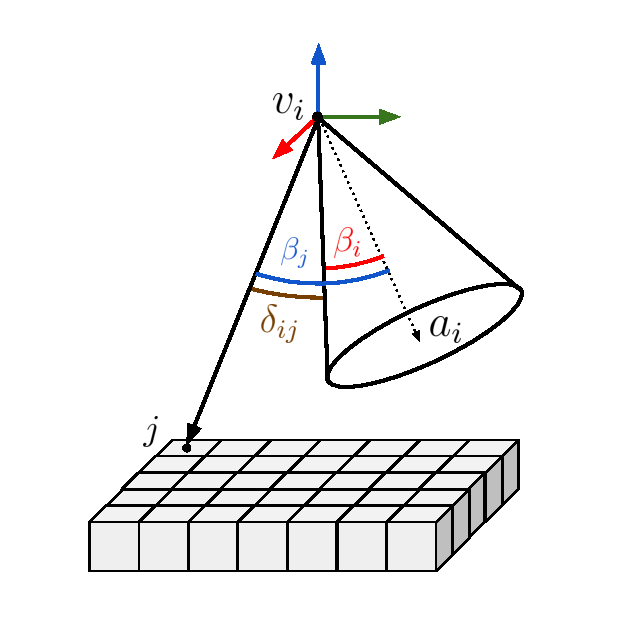
\includegraphics[width=0.4\textwidth]{./fig/photos/system_comp.eps}
    \caption{An illustration of the measurement $i$, which is composed of cone origin $v_{i}$, axis vector $a_{i}$ and Compton angle $\beta_{i}$.}
    \label{fig:system_comp}
\end{figure}
\subsubsection{Measurement noise}
The real-world measurements are affected by measurement noise. Hence the reconstructed cone might not intersect the real position of emission.
The measurement noise might be present in the measured energies $E_{1}$ and $E_{2}$ (that are affecting the Compton angle $\beta_{i}$ , see equation \autoref{eq:compton_beta_formula}) 
as well as in the positions of interactions inside the detector ($X_{1}$ and $X_{2}$) 
that are affecting the cone axis $a_{i}$.
The influence of noise in energy measurement (Compton angle $\beta$) is modelled using Gaussian function with ``standard deviation'' $\sigma$:
\begin{equation}
  h(\delta_{ij}|\sigma) = e^{-\frac{1}{2}(\frac{\delta_{ij}}{\sigma})^{2}}.
  \label{eq:gau}
\end{equation}
If the angle difference is large ($\delta_{ij}<3\sigma$), then we set $h(\delta_{ij}|\sigma) = 0$.
The important question is how to set the parameter $\sigma$, that is influencing the width of the function \autoref{eq:gau}.
The datasheet\footnote{Available at: https://advacam.com/camera/minipix-tpx3}
states that the energy resolution of used Timepix3 pixel detector is $4.5$--$9.9\ \mathrm{kEV}$. 
The dependence of angular uncertainties on the energy resolution of two-layer Compton cameras was studied in \cite{ordonez}.
The measurement of the energies is not the only source of noise in the detection pipeline.
The $h(\delta_{ij}|\sigma)$ function should disperse the conical back-projections in order to tackle other inaccuracies, such as noise in the sensor's position or wrongly estimated axis of the Compton cone. 
The exact estimation of angular uncertainty (and other sources of noise) is beyond the scope of this thesis.
%Other sources of noise (such as positions of interaction inside the detector $X_{1}$, $X_{2}$, especially depth of interaction in the sensor block) are difficult to model as well.
For ``proof of concept'' demonstration, the value $\sigma$ was set empirically based on recorded data from experiments with real \ac{pix} sensors.

\subsubsection{Discretization error}
Another possible source of noise is the discretization of the area of interest, which is divided into $J$ discrete bins (each represented by its centre position) with resolution $r$.
Even perfectly measured and reconstructed Compton cone might not intersect the real position of emission (meaning $\delta_{ij}$ would be non-zero) due to the discretization of $J$.
Let us define maximal error for measurement $i$ and position $j$ caused by discretization as
\begin{equation}
  \alpha_{ij} = \mathrm{arctan}(\frac{x}{d_{jv_{i}}}),
  \label{eq:alpha}
\end{equation}
where $d_{jv_{i}}$ is the distance between cone origin at position $v_{i}$ and map position $j$ and $x$ is the maximal allowed distance between projected cone and discrete position $j$, $x = l$.
The situation is illustrated in  \autoref{fig:discret}.
\begin{figure}
  \centering
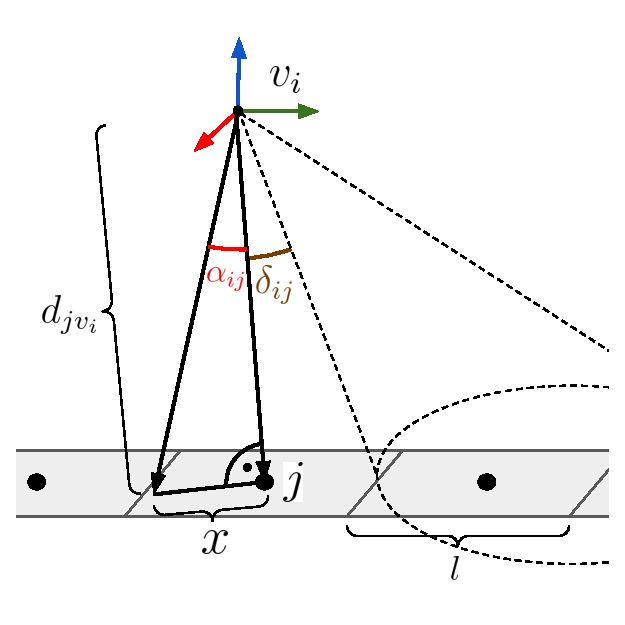
\includegraphics[width=0.4\textwidth]{./fig/photos/discret.eps}
  \caption{ 
Illustration of discretization error. The maximal angle difference caused by discretization error $\alpha_{ij}$ is computed for each map position $j$.}
  \label{fig:discret}
\end{figure}
Taking into account the discretization as well as measurement noise, the term $h(\delta_{ij}|\sigma, \alpha_{ij})$ in equation \autoref{eq:system_matrix_full} which is projecting the cone to the map positions is defined as
\begin{equation}
h(\delta_{ij}|\sigma) =
\begin{cases}
1 & \text{if $\delta_{ij}\leq \alpha_{ij}$}\\ 
e^{- \frac{1}{2}(\frac{\delta_{ij}}{\sigma})^{2}} & \text{if $\delta_{ij} > \alpha_{ij}$ and  $\delta_{ij} \leq 3\sigma_{j}$} \\
0 & \text{otherwise}
\end{cases}, 
\end{equation}
where $\alpha_{ij}$ is the maximal angle difference caused by discretization error defined in equation \autoref{eq:alpha}.








































%%%%%%%%%%%%%%%%%
%%%%%%%%%%%%%%%%%%%%
%%%%%%%%%%%%%%%%%%%%%
%%%%%%%%%%%%%%%%%%%%
%%%%%%%%%%%%%%%%
%%%%%%%%
%%%%%%%%%%
%%%%%%%%%%
%%%%%%%%%%%%
%%%%%%%%%%%%%%
%%%%%%%%%%%%
%

